\documentclass{article}
\usepackage{geometry}
 \geometry{
 a4paper,
 total={170mm,257mm},
 left=20mm,
 top=20mm,
 }
\usepackage{tgheros}
\usepackage[utf8]{inputenc}
\usepackage[english]{babel}
%\usepackage[english]{isodate}
%\usepackage[parfill]{parskip}
\usepackage[hybrid]{markdown}
\markdownSetup{
  pipeTables,
  tableCaptions,
  rendererPrototypes = {
    image = {\begin{center}\setkeys{Gin}{width=.99\linewidth}\includegraphics{#2}\end{center}}, % center images inline expanding to page width
    codeSpan = {\texttt{#1}}, % Render inline code via `\texttt`.'
  }
}
\title{AmpliPi Home Audio Controller - User Manual}
\author{MicroNova}
\date{November 2022}
\setlength\parindent{0pt}
\begin{document}

\maketitle
\setkeys{Gin}{width=.99\linewidth}
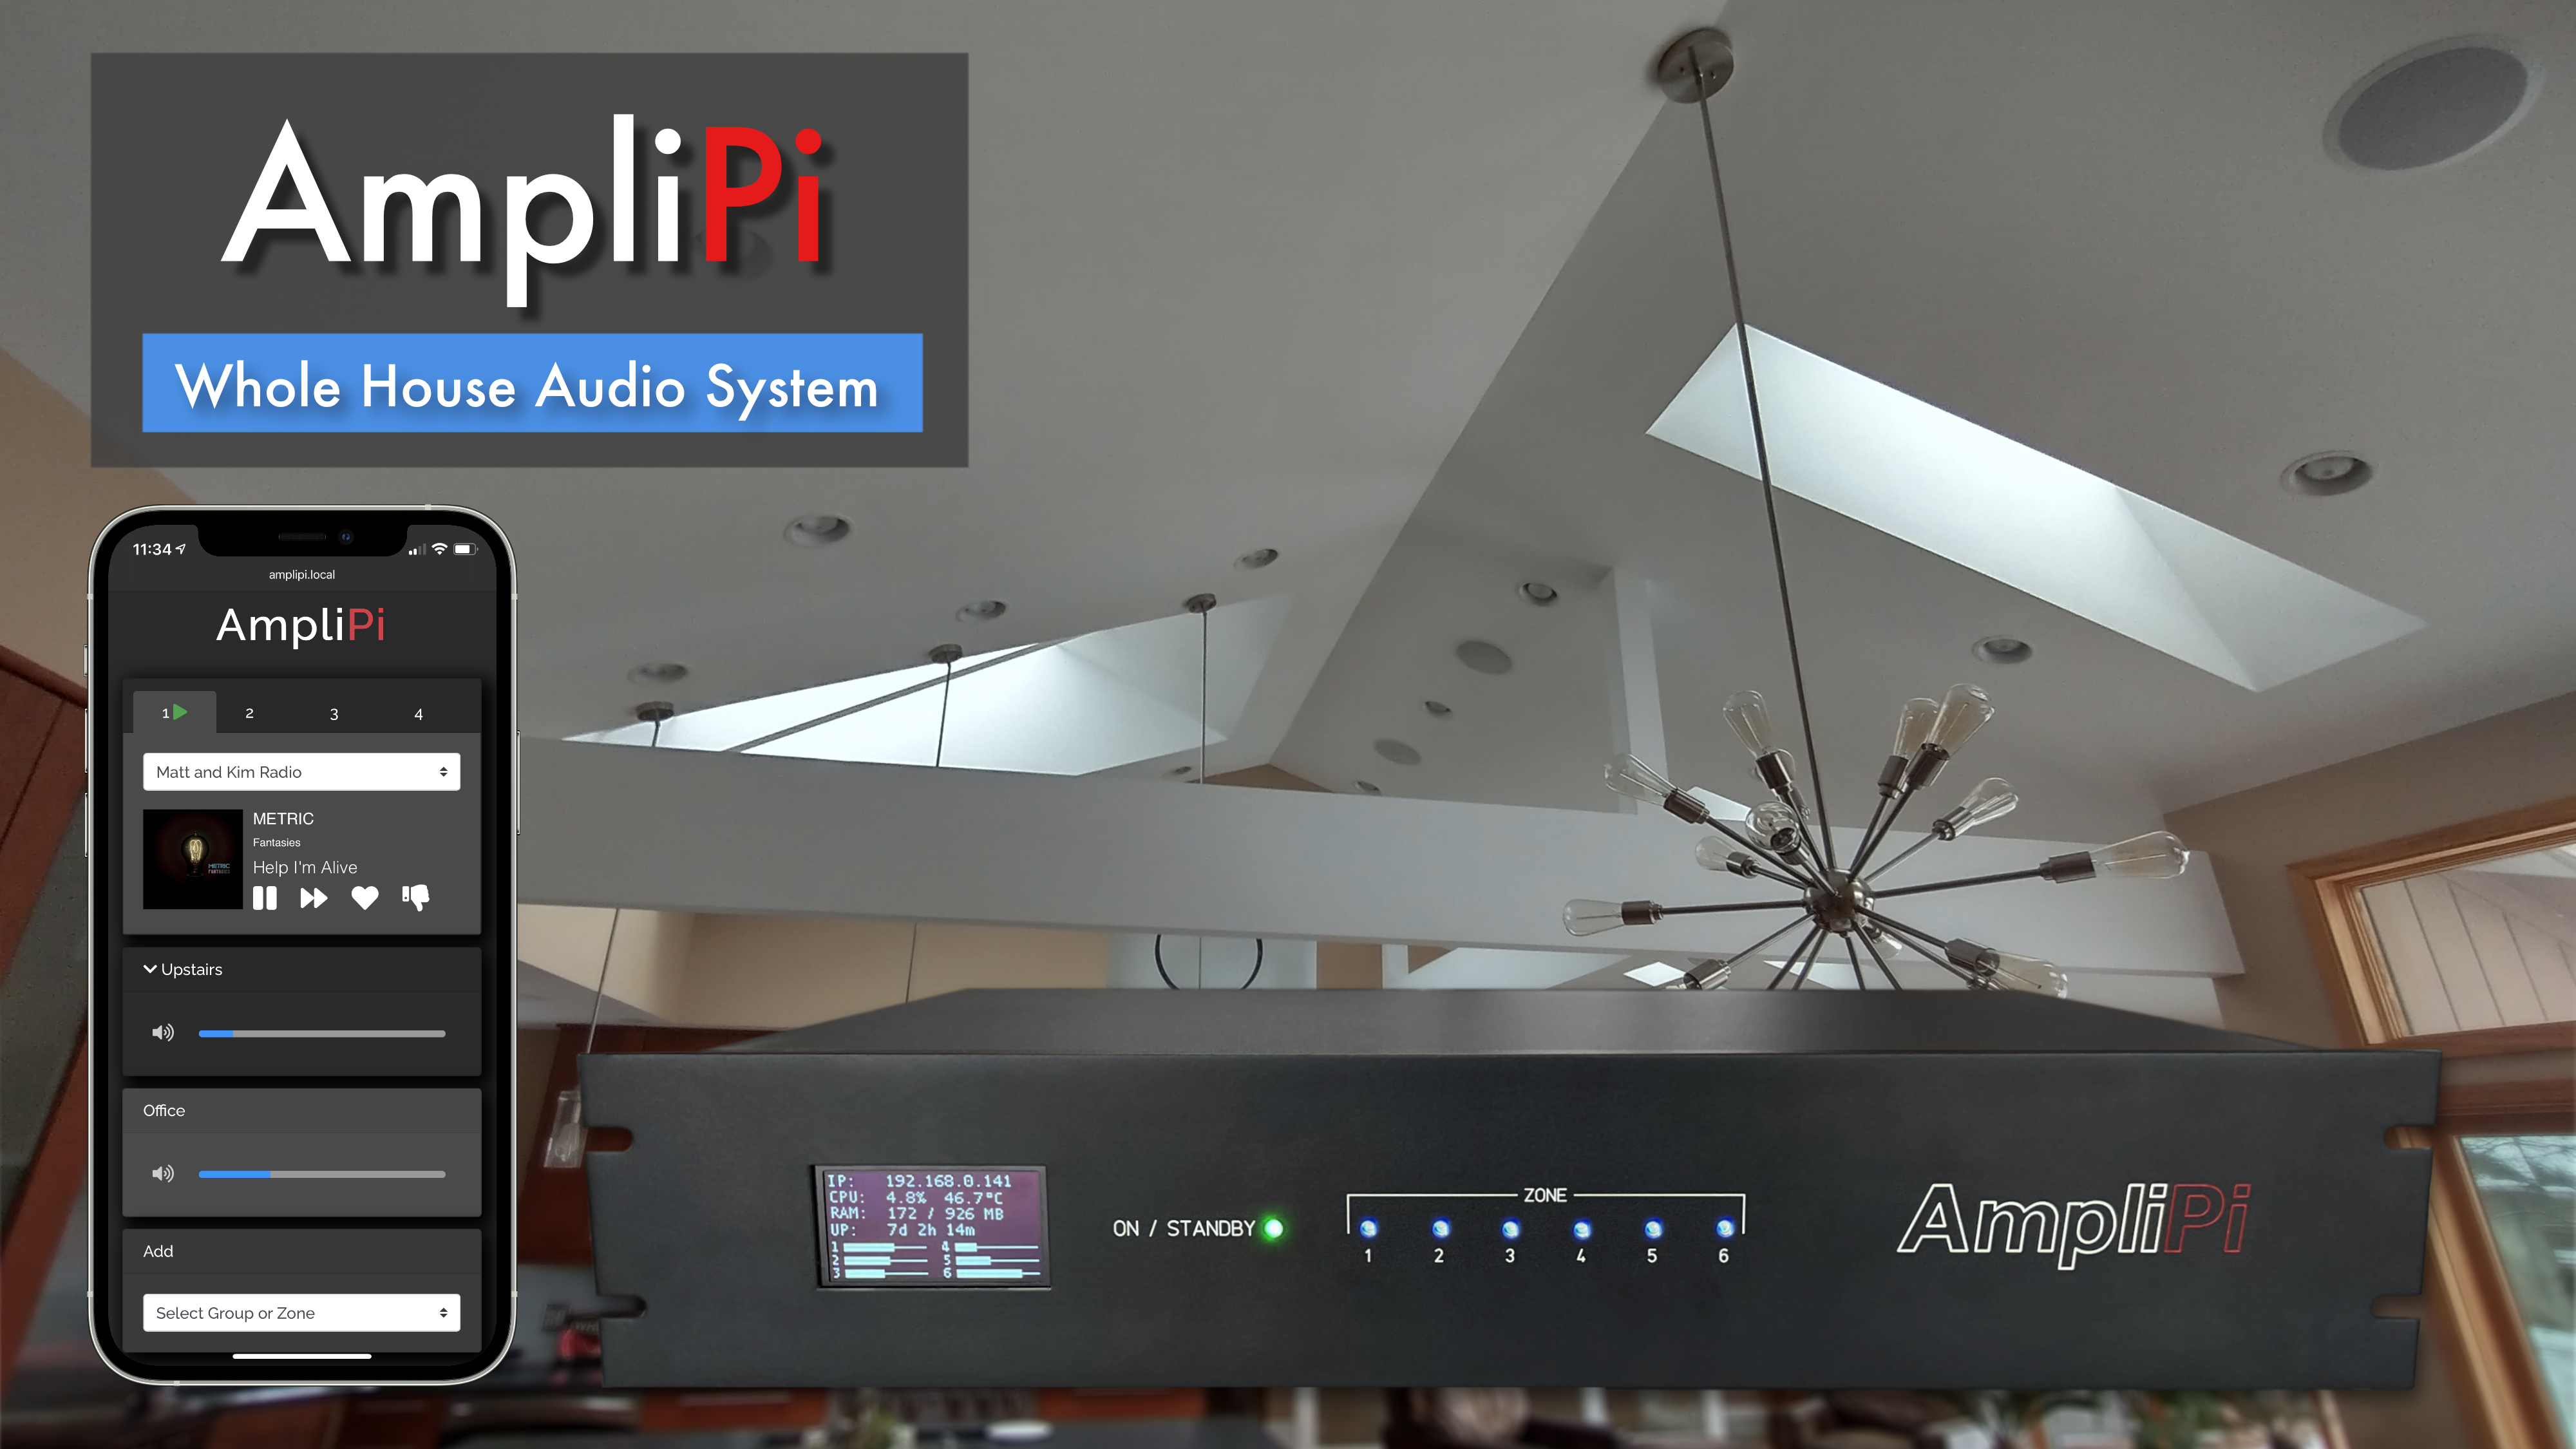
\includegraphics{imgs/manual/main_graphic_16x9.jpg}
\newpage

\pagenumbering{Roman}
\tableofcontents
\newpage
\pagenumbering{arabic}

\markdownInput{SAFETY.md}
\newpage
\markdownInput{FCC.md}
\newpage
\markdownInput{OVERVIEW.md}
\newpage
\markdownInput{MAIN_CONTROLLER.md}
\newpage
\markdownInput{MAIN_CONTROLLER_SPECS.md}
\newpage
\markdownInput{ZONE_EXPANDER.md}
\newpage
\markdownInput{ZONE_EXPANDER_SPECS.md}
\newpage
\markdownInput{WALL_PANEL.md}
\newpage
\markdownInput{INSTALLATION.md}
\newpage
\markdownInput{TROUBLESHOOTING.md}

\end{document}
